%%% LaTeX Template: Two column article
%%%
%%% Source: http://www.howtotex.com/
%%% Feel free to distribute this template, but please keep to referal to http://www.howtotex.com/ here.
%%% Date: February 2011

%%% Preamble
\documentclass[	DIV=calc,%
paper=a4,%
fontsize=12pt,%
onecolumn]{scrartcl}	 					% KOMA-article class
\usepackage{multicol}							%Texto em duas colunas
\usepackage{lipsum}			\usepackage{booktabs}										% Package to create dummy text
\usepackage[brazil]{babel}										% English language/hyphenation
\usepackage[protrusion=true,expansion=true]{microtype}				% Better typography
\usepackage{amsmath,amsfonts,amsthm}					% Math packages
\usepackage[pdftex]{graphicx}									% Enable pdflatex
\usepackage[svgnames]{xcolor}									% Enabling colors by their 'svgnames'
\usepackage[hang, small,labelfont=bf,up,textfont=it,up]{caption}	% Custom captions under/above floats
\usepackage{epstopdf}												% Converts .eps to .pdf
\usepackage{subfig}													% Subfigures
\usepackage{booktabs}												% Nicer tables
\usepackage{fix-cm}													% Custom fontsizes
\usepackage[utf8]{inputenc}
\usepackage[top=2.5cm, bottom=2.5cm, left=2.5cm, right=2.5cm]{geometry}
\usepackage[ddmmyyyy]{datetime}
\addto\captionsenglish{%
	\renewcommand\tablename{Tabela}
	\renewcommand\figurename{Figura}
} 



%%% Custom sectioning (sectsty package)
\usepackage{sectsty}													% Custom sectioning (see below)
\allsectionsfont{%															% Change font of al section commands
	\usefont{OT1}{phv}{b}{n}%										% bch-b-n: CharterBT-Bold font
}

\sectionfont{%																% Change font of \section command
	\usefont{OT1}{phv}{b}{n}%										% bch-b-n: CharterBT-Bold font
}



%%% Headers and footers
\usepackage{fancyhdr}												% Needed to define custom headers/footers
\pagestyle{fancy}														% Enabling the custom headers/footers
\usepackage{lastpage}	

% Header (empty)
\lhead{}
\chead{}
\rhead{}

\lfoot{\footnotesize \texttt{Cabeamento estruturado} \textbullet ~Juushin SA}


\cfoot{}
\rfoot{\footnotesize página \thepage\ de \pageref{LastPage}}	% "Page 1 of 2"
\renewcommand{\headrulewidth}{0.0pt}
\renewcommand{\footrulewidth}{0.4pt}



\usepackage{lettrine}
\newcommand{\initial}[1]{%
	\lettrine[lines=3,lhang=0.3,nindent=0em]{
		\color{DarkGoldenrod}
		{\textsf{#1}}}{}}



\usepackage{titling}															% For custom titles

\newcommand{\HorRule}{\color{DarkGoldenrod}%			% Creating a horizontal rule
	\rule{\linewidth}{1pt}%
}

\pretitle{\vspace{-30pt} \begin{flushleft} \HorRule 
		\fontsize{50}{50} \usefont{OT1}{phv}{b}{n} \color{DarkRed} \selectfont 
	}
	
	
	
	\title{Projeto de cabeamento estruturado para Juushin SA}					
	
	
	
	\posttitle{\par\end{flushleft}\vskip 0.5em}

\preauthor{\begin{flushleft}
		\large \lineskip 0.5em \usefont{OT1}{phv}{b}{sl} \color{DarkRed}}
	\author{Fernando Rocha }  	% Author name goes here
	
	
	\postauthor{\footnotesize \usefont{OT1}{phv}{m}{sl} \color{Black} 
		\\Universidade Tecnológica Federal do Paraná - Câmpus Cornélio Procópio 								% Institution of author
		\par\end{flushleft}\HorRule}

\date{}																				% No date




%%% Begin document
\begin{document}
	\maketitle
	\thispagestyle{fancy} 	
	\thispagestyle{empty}		% Enabling the custom headers/footers for the first page 
	
	\initial{O}\textbf{ presente documento tem como propósito colocar em prática o aprendizado da disciplina de cabeamento estruturado, criando uma estrutura de rede para uma empresa fictícia com base nas normas técnicas nacionais e internacionais, assim como as melhores práticas do seguimento.}
	
	
	\begin{figure}
		\centering
		
\includegraphics{utfpr}
	\end{figure}
	
	\vspace{2cm}
	\centerline{\textit{\textbf{\today}}}
	
	\clearpage
	\renewcommand*\listfigurename{Lista de figuras}
	\listoffigures
	
	\renewcommand*\listtablename{Lista de tabelas}
	\listoftables
	
	
	
	
	\clearpage
	\renewcommand{\contentsname}{Sumário}
	\tableofcontents
	\clearpage
	
	
	\section{Introdução}
	A Juushin SA é uma empresa que atua no área de serviços e conta, atualmente, com um quadro de 25 pessoas, sendo 9 que atuam na sede da empresa; 3 equipes de 5 pessoas, mais 1 Supervisor de equipe que atuam fora da sede. Atualmente a empresa está mudando sua sede para um novo prédio, portanto todo cabeamento será configurado a partir deste projeto.
	
	\subsection{Benefícios}
	
	O planejamento de um sistema de cabeamento traz vários benefícios às empresas que o adotam, dentre eles:
	\begin{itemize}
		\item Unifica a estrutura de dados, voz e vídeo reduzindo custos com manutenção e necessidade de atualização.
		\item Menor propensão a falhas, interrupções e interferências.
		\item Uma estrutura centralizada torna as alterações, que por ventura precisem ser feitas, mais rápidas e eficientes.
		\item Diminui drasticamente a inatividade do sistema, pois o diagnóstico de problemas é mais fácil que em uma rede não estruturada.
		\item O cabeamento estruturado tem maior durabilidade, pois sofre menos manipulação e tem melhor acondicinamento. 
	\end{itemize}
	\subsection{Organizações Envolvidas}
	\begin{table}[h!] % coloque h! para forcar a posicao
		\centering
		\caption{Organizações}
		\label{tab1} %com este label vc faz referencia no texto
		\begin{tabular}{llllll}
			\toprule
			{\textbf{EMPRESA}} & {\textbf{SERVIÇO}} & {\textbf{RESPONSÁVEL}} \\
			\midrule 
			Copel Telecom  & Provedor de Internet          & Mévio \\ 		
			BH Construtora & Piso e Instalação das calhas  & Caio\\ 
			VyperNET       & Montagem Racks e cabos        & Tício \\ 
			Certfik       & Certificação do Cabeamento     & Plinio \\
			\bottomrule
		\end{tabular}
	\end{table}
	
	
	
	\section{Estado atual}
	Hoje, a rede da empresa encontra-se na seguinte situação:
	\begin{itemize}
		\item 1 Switch 24 portas HP 1420-24G-2SFP, 2 Switches HP 1420-8G JH329A, 500m de cabos cat5e e 1 roteador Wireless D-Link DIR-615 N .
		\item As principais reclamações dos usuários são as quedas constantes e lentidão da conexão e a demora para impressão de documentos. Aproveitando a construção da nova sede, os diretores optaram por fazer um projeto de cabeamento estruturado.
	Após análise da rede foi possível encontrar vários pontos que possam estar ocasionando os problemas relatados pelos usuários, entre eles:
		\item Cabos de rede e elétricos acondicionados juntos;
		\item Cabos de rede dobrados ou retorcidos;
		\item Cabos de rede sem identificação;		
		\item Conectores não padronizados;
		\item Switch com portas danificadas;
	\end{itemize}
	
	\section{Requisitos}
	A nova estrutura de rede deve eliminar os problemas atuais de conexão e ainda:
	\begin{itemize}
		\item Padronizar toda a estrutura de rede.
		\item Identificar os cabos.
		\item Separar o cabeamento de rede do cabeamento elétrico.
		\item Acondicionar adequadamente os equipamentos de rede.
		\item Atender demanda atual de rede e futuras expansões.				
	\end{itemize}	
	
	\section{Usuários e Aplicativos}
	Atualmente a empresa tem como usuários seus 25 colaboradores mais os clientes que fazem uso da rede sem fio. Com a crescente demanda por serviços este número pode aumentar nos próximos anos, por isso é importante que o projeto preveja uma possível expansão da rede atual.
	
	\begin{multicols}{2}
	\subsection{Usuários}
	\begin{itemize}
		\item Diretores: 3;
		\item Atendentes: 2;
		\item Administrativo: 4;
		\item Membros das Equipes: 15;
		\item Clientes: até 20;
	\end{itemize}
	\subsection{Aplicativos}
	\begin{itemize}
		\item Sistema ERP: 9;
		\item Pacote Office: 9;
		\item Sistema de Vendas: 4;
		\item Software Contábil: 1;
	\end{itemize}
	\end{multicols}{2}
	\section{Estrutura predial existente}
	Como a empresa está transferindo sua sede para um novo prédio, não convém falar sobre a estrutura predial existente. Este documento discorrerá apenas sobre a nova estrutura.
	%inicio dos comandos para criar uma nova pagina A3 horizontal
	\clearpage
	\KOMAoptions{paper=a3, paper=landscape, DIV=20}
	\recalctypearea
	
	\begin{figure}
		%	\centering
		\noindent\makebox[\textwidth][c]{
			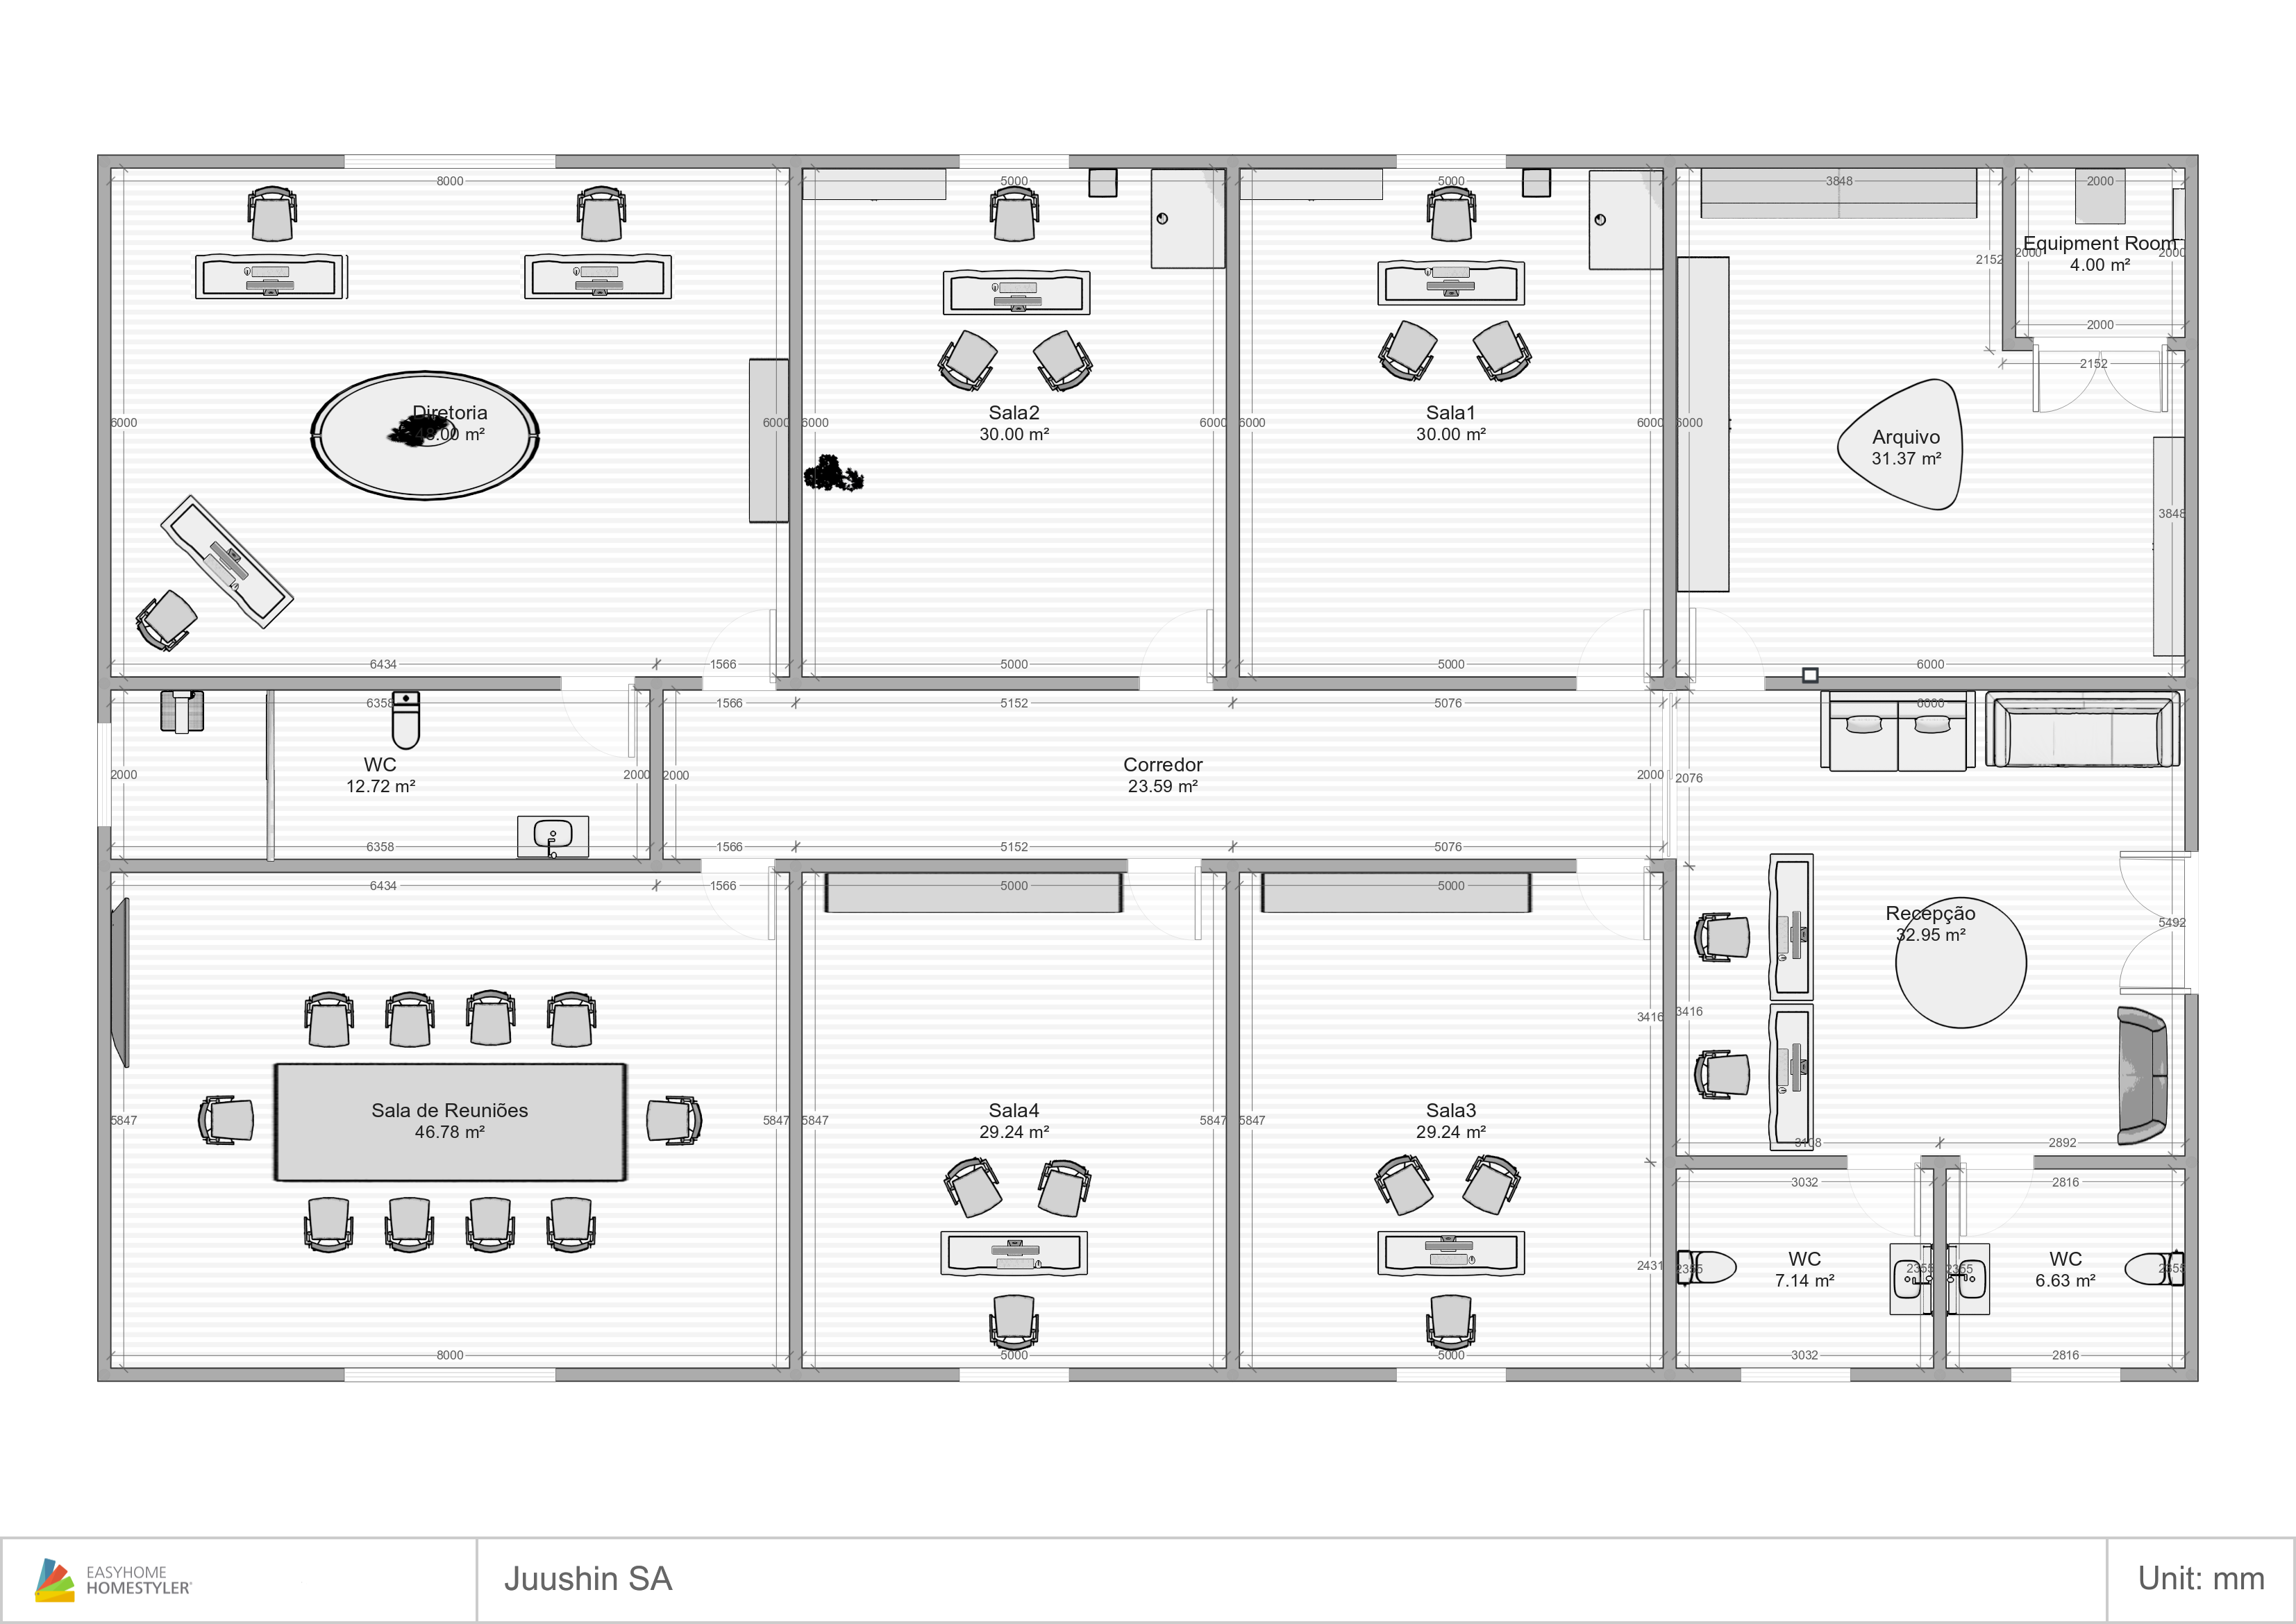
\includegraphics[width=\textwidth]{fig1}
		}
		\caption{Planta física}
		\label{fig1}
	\end{figure}
	
	%Retornar ao formato A4
	\clearpage
	\KOMAoptions{paper=a4, paper=portrait, DIV=calc}
	\recalctypearea
	%-- reinicio em A4 
	
	\section{Planta Lógica - Elementos estruturados}
	
	\subsection{Topologia}
	
		A planta da nova sede conta com uma sala de recepção com $ 32,95m^{2}  $ e 4 pontos de rede com espaçamento de 2 metros; quatro salas administrativas com aprox. $ 30m^{2}  $ e 5 pontos de rede com espaçamento de 2 metros; uma sala de diretores com $ 48m^{2}  $ e 6 pontos de rede com espaçamento de 2 metros; uma sala para reuniões com $ 46,78m^{2}  $ e 8 pontos de rede com espaçamento de 2 metros;  3 banheiros e uma sala de arquivos com $ 31,37m^{2}  $ e 4 pontos de rede com espaçamento de 2 metros, onde se encontra a sala de equipamentos.
		
		\begin{figure}[h]
			\centering	
			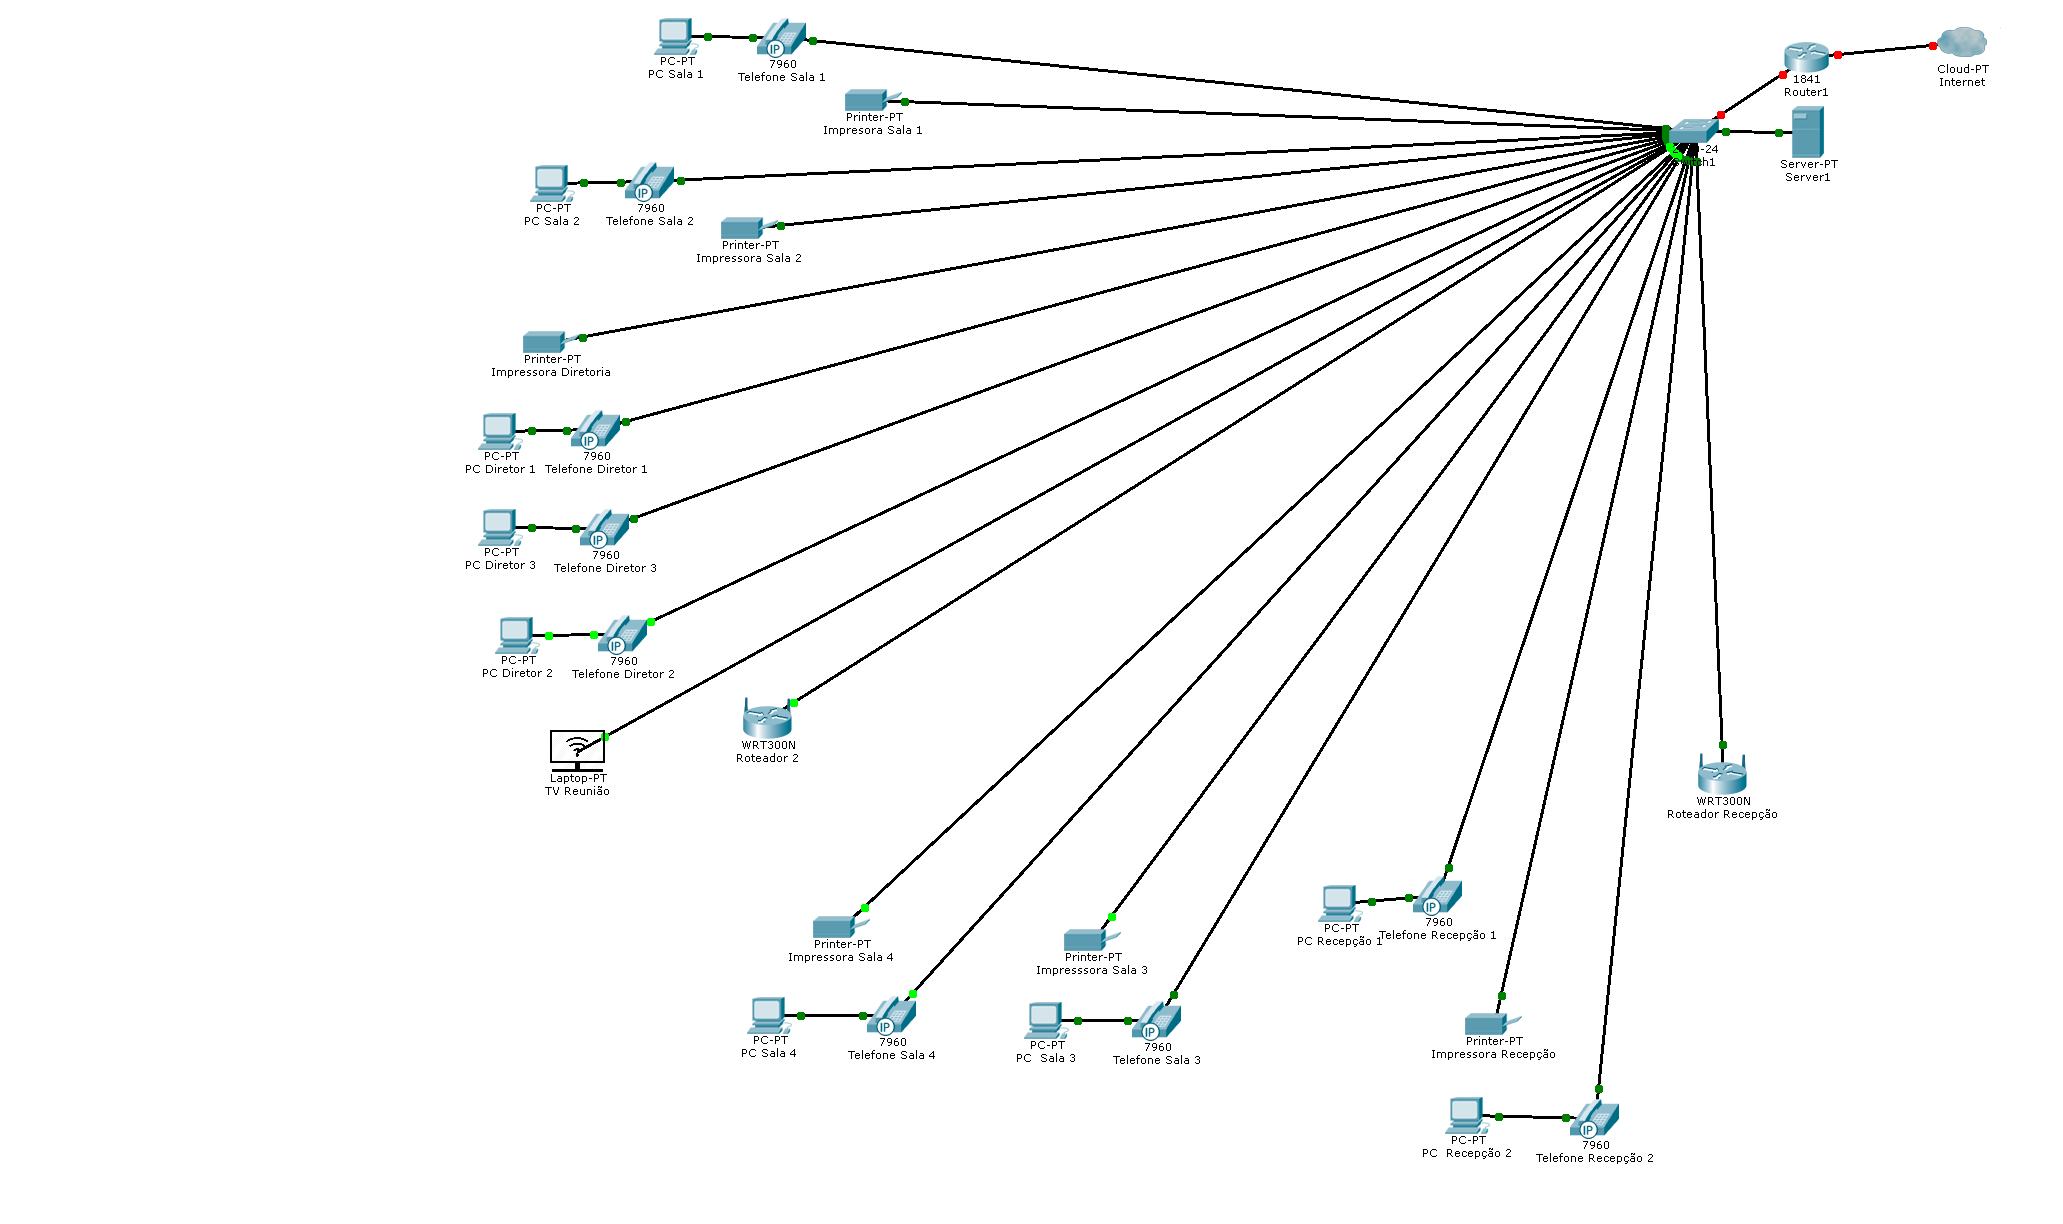
\includegraphics[width=\textwidth]{fig2}
			\caption{Planta Lógica}
			\label{fig2}
		\end{figure}
	
	\subsection{Encaminhamento}
	Os cabos seguirão em eletrocalhas sob o piso elevado e sairão por eletrodutos até as tomadas, localizadas a 0,45m acima do piso. A Eletrocalha "A", identificada no projeto com a cor azul, conterá o cabeamento da sala 1, sala 2 e sala da diretoria, totalizando 14 cabos, conforme NBR 16415 \cite{ref1}.
	A eletrocalha "B", identificada no projeto com a cor vermelha, conterá o cabeamento da sala 3, sala 4 e sala de reuniões.	A eletrocalha "C", de cor verde, conterá o cabeamento da sala de arquivos, recepção, sala 3, sala 4 e sala de reuniões. 
	
	
	%inicio dos comandos para criar uma nova pagina A3 horizontal
	\clearpage
	\KOMAoptions{paper=a3, paper=landscape, DIV=20}
	\recalctypearea
	
	\begin{figure}
		%	\centering
		\noindent\makebox[\textwidth][c]{
			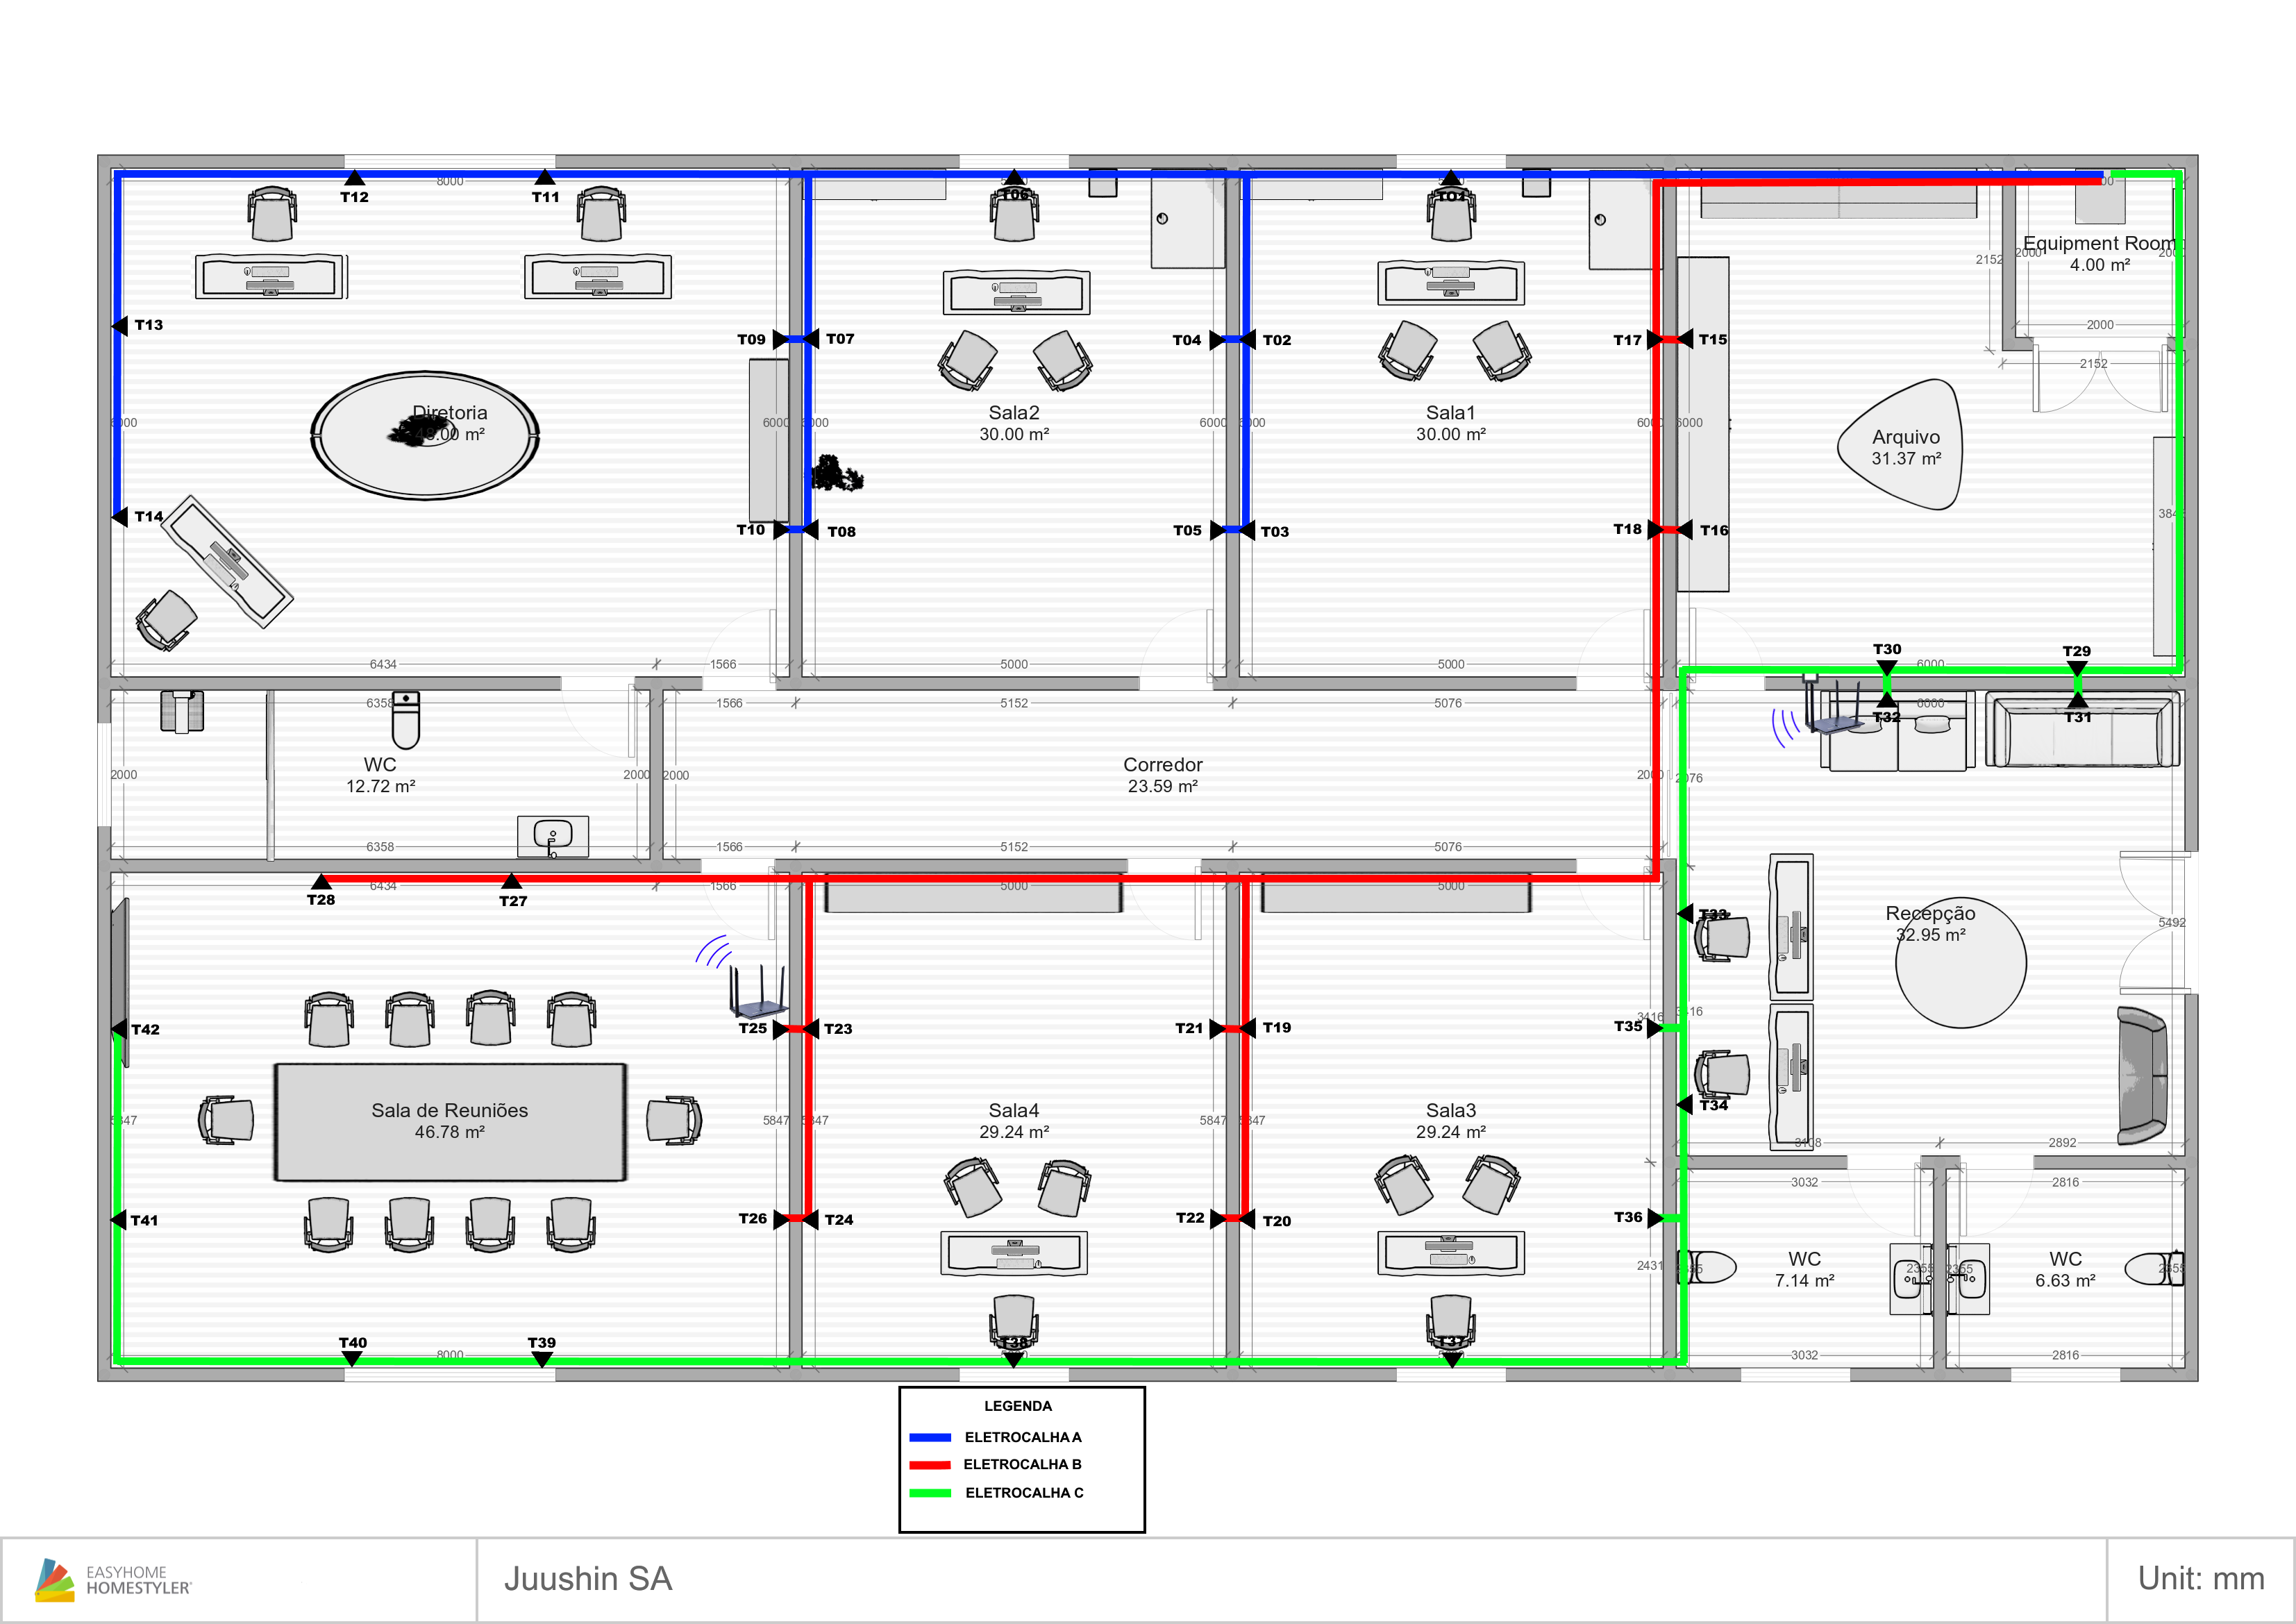
\includegraphics[width=\textwidth]{fig3}
		}
		\caption{Encaminhamento}
		\label{fig3}
	\end{figure}
	
	%Retornar ao formato A4
	\clearpage
	\KOMAoptions{paper=a4, paper=portrait, DIV=calc}
	\recalctypearea
	%-- reinicio em A4 
	\subsection{Memorial descritivo}
	
\begin{table}[h!]
	\footnotesize
	\centering
	\caption{Componentes Utilizados}
	\label{tab2} %com este label vc faz referencia no texto
	\begin{tabular}{lll}
		\toprule
		{\textbf{COMPONENTE}} & {\textbf{FABRICANTE}} & {\textbf{QUANTIDADE}} \\
		\midrule
		Abraçadeira Nylon 2,5 x 100mm c/100   & Western    & 5          \\
		Cabo De Rede Cat6 U/utp 305m          & Furukawa   & 3          \\
		Conector Rj45 Cat6 (pacote C/50)      & Furukawa   & 2         \\
		Eletrocalha 50x50 3m                  & Cemar      & 63         \\
		Eletrocalha Curva Horiz 90 50x50      & Cemar      & 8          \\
		Eletrocalha Te 90 50x50               & Cemar      & 4          \\
		Eletroduto Em Pvc c/ 3 Metros         & Tigre      & 7          \\
		Kit Cx+tampa+Tomada Rj45 Cat.6 10u    & Tramontina & 5          \\
		Patch Cord Cat6 1,5m Gigalan vermelho & Furukawa   & 50         \\
		Patch Cord Cat6 2,5m Gigalan vermelho & Furukawa   & 20         \\
		Patch Panel Cat.6 48 Posições         & Itcomtech  & 1          \\
		Rack para Servidor Fechado 44U        & Inforack   & 1          \\
		Régua tomadas c/ 12 Tomadas Bivolt    & Ipec       & 1          \\
		Roteador AC DIR-815                   & D-Link     & 2          \\
		Switch 48 portas                      & HP         & 1          \\
		\toprule
	\end{tabular}
\end{table}
	
	\subsection{Identificação dos cabos}

	De acordo com Pinheiro \cite{ref2}, cada unidade de terminação de hardware deve ter uma identificação exclusiva, conforme estabelece a norma ANSI/EIA/TIA - 606. Deste modo a identificação dos cabos seguirá o seguinte padrão:
	
	\subitem Txx - Ponto de comunicação
	\subitem W - Calha
	\subitem Pxx - Porta do Patch Panel
	\subitem Y - UTP(U), STP(S), FIBRA OTICA (Fo)
	\subitem Cxx - Número do cabo
	
	
    \textbf{Exemplo:} 
    
	\begin{figure}[h]
		\centering
		
		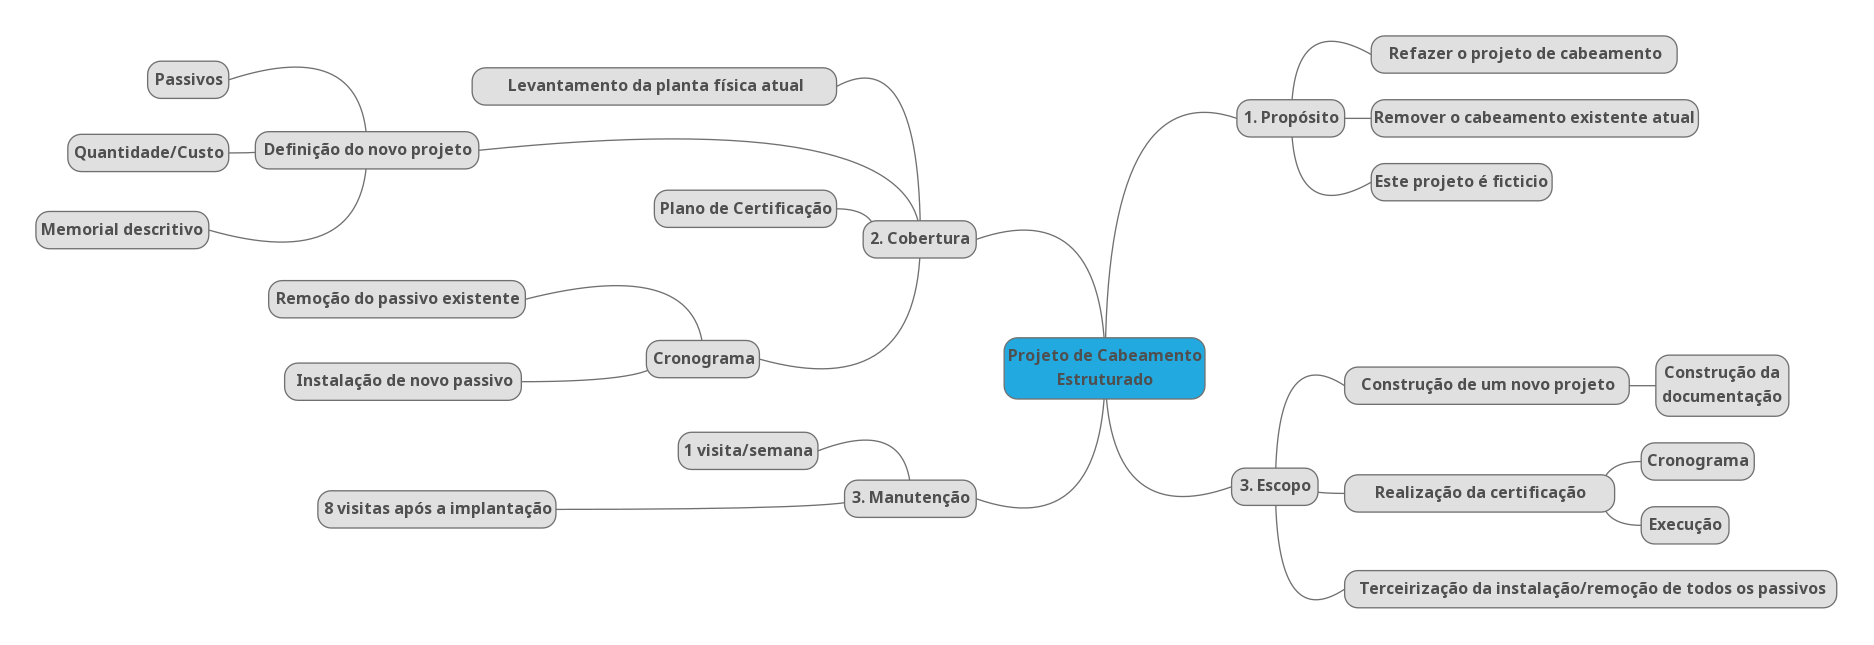
\includegraphics[width=4cm]{fig4}
		\caption{Identificação de Cabo}
		\label{fig4}
	\end{figure}
	A figura \ref{fig4} indica o cabo 01, que liga a porta 1 do Patch Panel ao Ponto de Telecomunicações 01, passando pela calha A no primeiro Andar. O tipo de cabo usado é UTP.
\clearpage	
\begin{table}[h]
	\footnotesize
	\centering
	\caption{Pontos de rede}	
	\label{tab3} %com este label vc faz referencia no texto
		\begin{tabular}{lllll}
			\toprule
			{\textbf{PONTO DE COMUNICAÇÃO}} & {\textbf{CALHA}} & {\textbf{PORTA}} & {\textbf{Nº CABO}} & {\textbf{DIST (M)}}    \\
			\midrule
		T01                  & A     & 1                 & 1        & 8        \\
		T02                  & A     & 2                 & 2        & 12.5     \\
		T03                  & A     & 3                 & 3        & 14.5     \\
		T04                  & A     & 4                 & 4        & 13       \\
		T05                  & A     & 5                 & 5        & 15       \\
		T06                  & A     & 6                 & 6        & 13       \\
		T07                  & A     & 7                 & 7        & 17.5     \\
		T08                  & A     & 8                 & 8        & 19.5     \\
		T09                  & A     & 9                 & 9        & 18       \\
		T10                  & A     & 10                & 10       & 20       \\
		T11                  & A     & 11                & 11       & 18       \\
		T12                  & A     & 12                & 12       & 21       \\
		T13                  & A     & 13                & 13       & 25.5     \\
		T14                  & A     & 14                & 14       & 27.5     \\
		T15                  & B     & 15                & 15       & 8        \\
		T16                  & B     & 16                & 16       & 10       \\
		T17                  & B     & 17                & 17       & 7.5      \\
		T18                  & B     & 18                & 18       & 9.5      \\
		T19                  & B     & 19                & 19       & 20.5     \\
		T20                  & B     & 20                & 20       & 22.5     \\
		T21                  & B     & 21                & 21       & 21       \\
		T22                  & B     & 22                & 22       & 23       \\
		T23                  & B     & 23                & 23       & 25.5     \\
		T24                  & B     & 24                & 24       & 27.5     \\
		T25                  & B     & 25                & 25       & 26       \\
		T26                  & B     & 26                & 26       & 28       \\
		T27                  & B     & 27                & 27       & 26.5     \\
		T28                  & B     & 28                & 28       & 29       \\
		T29                  & C     & 29                & 29       & 8        \\
		T30                  & C     & 30                & 30       & 10       \\
		T31                  & C     & 31                & 31       & 8.5      \\
		T32                  & C     & 32                & 32       & 10.5     \\
		T33                  & C     & 33                & 33       & 15.5     \\
		T34                  & C     & 34                & 34       & 16.5     \\
		T35                  & C     & 35                & 35       & 15       \\
		T36                  & C     & 36                & 36       & 17       \\
		T37                  & C     & 37                & 37       & 22       \\
		T38                  & C     & 38                & 38       & 27.5     \\
		T39                  & C     & 39                & 39       & 32.5     \\
		T40                  & C     & 40                & 40       & 35       \\
		T41                  & C     & 41                & 41       & 39.5     \\
		T42                  & C     & 42                & 42       & 41.5     \\
		\bottomrule
		\end{tabular}
	\end{table}
\clearpage	
	
	\section{Implantação}
A figura \ref{fig5} apresenta tabela com o cronograma de implantação previsto. O cronograma já engloba eventuais atrasos, assim a implantação deve ocorrer dentro de 4 semanas.
		\begin{figure}[h]
			\centering
			
			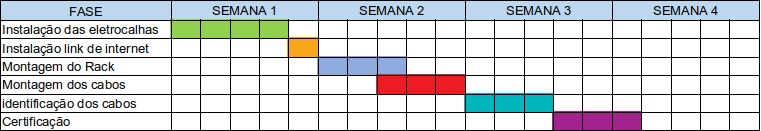
\includegraphics[width=\textwidth]{fig5}
			\caption{Cronograma de implantação}
			\label{fig5}
		\end{figure}
	
	\section{Plano de certificação}
Este projeto foi desenvolvido observando-se as normas técnicas vigentes, em especial a NBR 14565 \cite{ref3}, visando entregar uma estrutura de alta qualidade para o cliente. Com objetivo identificar quaisquer falhas decorrentes da instalação e obter o melhor desempenho de toda a estrutura de cabeamento será realizada, na semana final de trabalho, a certificação da rede, onde serão testados cabos, conectores, tomadas, patch cords e patch panel. O cabeamento deverá atender aos parâmetros de testes primários a seguir:
	\begin{itemize}
	\item Wiremap - Mapa de Fios;
	\item Atenuação de sinal;
	\item NEXT (Near-end Crosstalk) - Diafonia Próxima;
	\item PSNEXT (Power sum near-end crosstalk) - Diafonia próxima por soma de potências;
	\item ELFEXT (Equal-level far-end crosstalk) - Diafonia distante de mesmo nível;
	\item PSELFEXT(Power sum equal-level far-end crosstalk) - Diafonia distante por soma de potência de mesmo nível;
	\item Desvio de Atraso;
	\item Atraso de Propagação;
	\item Perda de Retorno;
	\item Comprimento do cabo;
	\end{itemize}
Toda a rede passará pelo processo de certificação e ao final será emitido relatório detalhado que será anexado à documentação a ser entregue ao cliente.
	
	\section{Plano de manutenção}
	
	O projeto atual prevê um plano de manutenção preventiva periódica  rede, que ocorrerá ao fim de cada semestre do primeiro ano de implantação da rede e após este período ao final de cada ano, a critério do cliente.
	
	\subsection{Plano de expansão}
	A empresa acaba de passar por um processo de expansão, mas tem se preparado para crescimentos futuros, por isso o projeto de rede atual já conta com pontos de comunicação sobressalentes e a própria estrutura predial já prevê uma possível ampliação para até 3 andares. A sala de equipamentos está localizada em um ponto onde será possível a criação de um backbone para esta  ampliação, sendo recomendado o uso de fibra ótica para este fim. O Rack atual já tem espaço para instalação de novos equipamentos que atendam a demanda futura.
	
	\section{Risco}
	A estrutura de rede em si não apresenta grandes riscos, uma vez que os cabos de rede passam sob o piso elevado, devidamente acondicionados dentro de eletrocalhas e longe do cabeamento elétrico. A sala de Equipamentos possui portas com trancas assim como o Rack onde ficarão os equipamentos, impedindo assim o acesso não autorizado. A sala de equipamentos possui refrigeração, pois está localizada dentro da sala de Arquivos, que possui também sistema de combate a incendios. A parte elétrica conta ainda com protetores de surto e o aterramento dos equipamentos de rede é separado do aterramento do prédio em si.
	
	\section{Orçamento}
	A tabela \ref{tab3} apresenta o orçamento do projeto, realizado na data de 28 de novembro de 2019 e com validade de 30 dias.
	\begin{table}[h!]
		\footnotesize
		\centering
		\caption{Custos do Projeto}
		\label{tab3} %com este label vc faz referencia no texto
	%	\begin{center}
		\renewcommand{\arraystretch}{1.5}
			\begin{tabular}{lllll}
				\toprule
				{\textbf{COMPONENTE/ SERVIÇO}}                   & {\textbf{EMPRESA}}        & {\textbf{QTDE}} & {\textbf{PREÇO}} & {\textbf{TOTAL}}   \\
				\midrule
				Abraçadeira Nylon 2,5 x 100mm c/100   & Western        & 5          & 1,83     & 9,15     \\
				Cabo De Rede Cat6 U/utp 305m          & Furukawa       & 3          & 590,00   & 1.770,00 \\
				Conector Rj45 Cat6 (pacote C/50)      & Furukawa       & 2          & 190,76   & 381,52   \\
				Eletrocalha 50x50 3m                  & Cemar          & 63         & 33,21    & 2.092,23 \\
				Eletrocalha Curva Horiz 90 50x50      & Cemar          & 8          & 18,15    & 145,20   \\
				Eletrocalha Te 90 50x50               & Cemar          & 4          & 23,48    & 93,92    \\
				Eletroduto Em Pvc c/ 3 Metros         & Tigre          & 7          & 12,99    & 90,93    \\
				Kit Cx+tampa+Tomada Rj45 Cat.6 10u    & Tramontina     & 5          & 144,28   & 721,40   \\
				Patch Cord Cat6 1,5m Gigalan vermelho & Furukawa       & 50         & 26,90    & 1.345,00 \\
				Patch Cord Cat6 2,5m Gigalan vermelho & Furukawa       & 20         & 37,90    & 758,00   \\
				Patch Panel Cat.6 48 Posições         & Itcomtech      & 1          & 435,00   & 435,00   \\
				Rack para Servidor Fechado 44U        & Inforack       & 1          & 1.673,76 & 1.673,76 \\
				Régua tomadas c/ 12 Tomadas Bivolt    & Ipec           & 1          & 33,90    & 33,90    \\
				Roteador AC DIR-815                   & D-Link         & 2          & 155      & 310,00   \\
				Switch 48 portas                      & HP             & 1          & 2.535,90 & 2.535,90 \\
				Instalação Link de Internet           & Copel          & 1          & 135      & 135,00   \\
				Instalação piso e eletrocalhas        & BH Construtora & 1          & 1.350,90 & 1.350,90 \\
				Montagem do Rack e Cabeamento         & VyperNET       & 1          & 1.500,00 & 1.500,00 \\
				Certificação da rede                  & Certifik       & 1          & 1.280,00 & 1.280,00 \\
				\bottomrule
				VALOR TOTAL                           &                &            &          & 16661,81\\
				\bottomrule
			\end{tabular}
	\end{table}
	
	\section{Recomendações}
	Recomenda-se manter o acesso à sala de equipamentos restrito exclusivamente aos colaboradores responsáveis pelos equipamentos de TI. Estes mesmos colaboradores devem relatar qualquer anormalidades encontradas na sala e nos equipamentos, bem como avaliar a necessidade de limpeza do local.
	
	\section{Referências bibliográficas}
	\renewcommand\refname{} %%Referências bibliográficas}  
	\bibliographystyle{ieeetr}
	\bibliography{referencias}  

\end{document}	
